P2P networks can have various topography based on how much they want to be decentralized.

\section{Semi-decentralized systems}
Napster is the most famous example of semi-decentralized system, the basic idea is to use proprietary server to exchange information about files, but then in order to actually exchange those files, the users had to connect directly one to each other.
Centralized servers are used to store indexes to files only.
This topology allows to decrease the consumption of bandwidth by those server allowing at the same time for large sharing.

In Napster we see for the first time the term \emph{peer} referring to an entity that both provide the service and uses it, and with that the term \emph{peer-to-peer system}.

Strengths of this solution:
\begin{itemize}
    \item it's great for resource sharing;
    \item each node pays its participation by providing access to its resources;
    \item each node is a peer;
    \item global information without huge investments (a single server can serve a lot of users);
    \item decentralization of costs and administration avoiding resource bottlenecks.
\end{itemize}

Weaknesses of this solution:
\begin{itemize}
    \item those servers are still a single point of failure;
    \item unique entity required for controlling the system;
    \item copying copyrighted material made Napster target of legal actions cause it was the owner of the indexes.
\end{itemize}

\section{Fully-decentralized systems}
Gnutella reuses the idea to store files on the peers, but now avoiding the existence of a central index.
Moreover peers establish non transient direct connections between themselves not for content sharing but only for sharing.

\subsection{Overlay network}
An overlay network is a virtual network built on physical one.
Overlay links are tunnels through the underlying network, not all logical links are also physical so each logical link can be a direct connection or traverse any set of routers.
Overlay network are usually implemented at the application layer.

\begin{figure}[H]
    \centering
    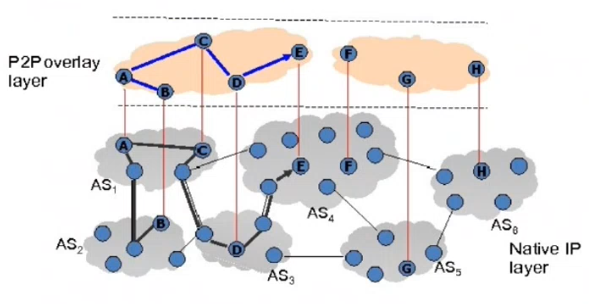
\includegraphics[width=330px]{images/2_p2p_networks/01.png}
    \caption{Overlay network}
\end{figure}

\subsection{P2P protocol}
A protocol is a set of rules, and of course a p2p protocol defines the set of messages that the peers exchange, both their format and their semantics.
Moreover a p2p protocol is defined over a p2p overlay.
Some definition regards:
\begin{itemize}
    \item routing strategies at the application level;
    \item identification of the peer through unique identifiers, generally computed through a hash function;
    \item headers and payloads format.
\end{itemize}

\section{Classification of p2p overlays}
\subsection{Unstructured overlay}
In an unstructured overlay peers are arbitrarily connected, so the result is an unstructured network.
In order to execute a search in that network we can exploit \emph{flooding} and \emph{expanding ring} or \emph{random walk}.

This structure is easy to code and maintain, it's high resilient due to the high number of connections for each peer, but it has high lookup cost because in the worst case you have to ask for a resource to each node, since there is no way to direct index information, moreover it doesn't scale well.

Some example of those overlay are:
\begin{itemize}
    \item Gnutella up to v0.4;
    \item BitTorrent, before switching to DHT;
    \item BitCoin
\end{itemize}

\subsubsection{Gnutella}
In Gnutella there is no information indexing and connections are defined at random.
In order to join the network it is possible to query a known DNS servers which contains IP addresses of a set of \emph{stable peers}.
This server collects peers and dynamically and automatically updates its cache in order to rank for stability.
Moreover for a peer it is possible to use an internal cache to store IP addresses of peers contacted in current and previous sessions, of course updating it by talking with neighbour peers.

\subsubsection{Flooding and TTL Enhanced flooding}
\begin{itemize}
    \item step 0: join the network;
    \item step 1: determine who is on the network, mainly by:
    \begin{itemize}
        \item sending \emph{ping} message to announce your presence on the network;
        \item other peers both respond with a \emph{pong} message and forward the ping one to other connected peers;
        \item the pong packet contains info on the peer sending it;
    \end{itemize}
    \item step 2: searching by asking other peer for some content.
    If one of the contacted peer has the resource it will respond, otherwise it will send the query packet to its other neighbours.
    Of course this flooding must be limited using a TTL to avoid infinity packet traverse and by using unique identifier on the messages to avoid cycles.
    \item step 3: download via direct connection from the requester to who has the match.
\end{itemize}
NB: the response to a query is forwarded using \emph{backward routing} so the response makes the exact same hops as the request message, but backward.
Once the response reaches the requester then it issues a direct connection to the peer who holds the resource.

\begin{figure}[H]
    \centering
    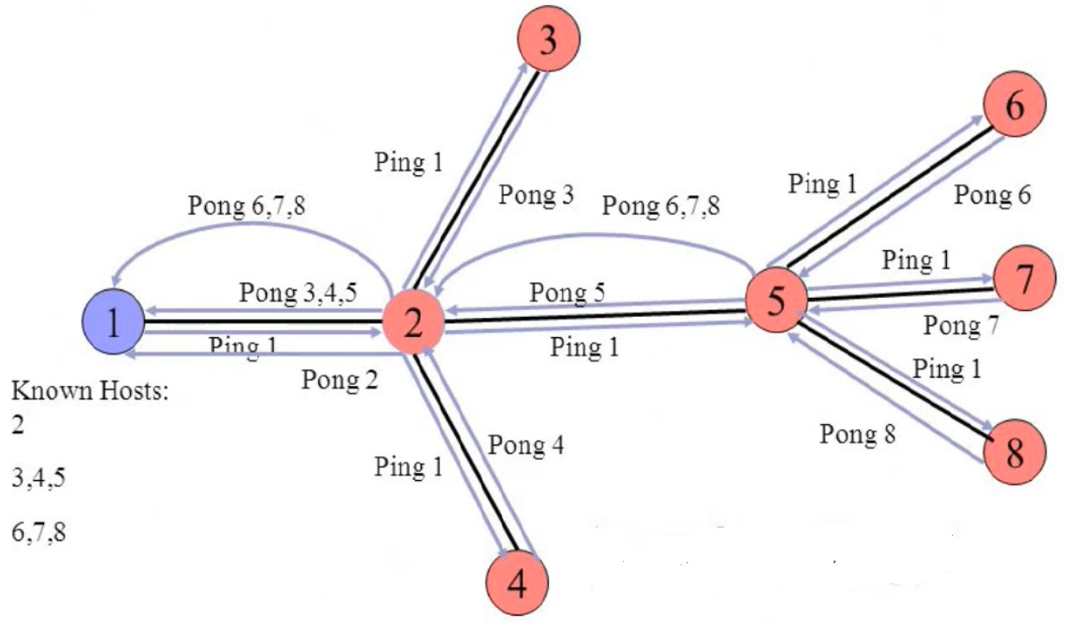
\includegraphics[width=330px]{images/2_p2p_networks/02.png}
    \caption{Ping pong protocol}
\end{figure}

The content detection is not guaranteed.
In particular false negatives may occur due to the TTL that limits the propagation of search and information, moreover the TTL stuff reduces the scalability.

However it is one of the most used algorithm in unstructured p2p networks.

\subsubsection{Expanding ring or iterative deepening}
To avoid packet flooding in a network a peer can apply a breadth first search by issuing a sequence of flood with increasing TTL.
Use only a subset of neighbors (maybe chosen at random or based on an heuristic), start a BFS with a low TTL value and if the search is not succesfull then repeat the BFS increasing the TTL (and so the depth of the search).

\subsubsection{Random walk}
Random walk (or drunkard's walk) uses a path constructed by taking successive steps in random directions.
This process is described by a \emph{Markov chain} which is a mathematical structure that is used to study probability distribution in memory-less system.

The idea of the algorithm is to run $k$ query messages, each of them will perculate a random walk (with a probabilistic protocol) of the same distance.
Each path is called a \emph{walker}.

This search algorithm reduces the number of messages avoiding an exponential explosion but of course the latency increases.
It uses two methods to terminate each walker:
\begin{itemize}
    \item TTL
    \item checking method: the walker periodically check with the query source if the stop condition has been met.
\end{itemize}

To increase the efficiency of the protocol we can think of bias the walks towards high-degree nodes, this way we can increase the probability of finding the resource.

In the end the protocol performance depends on parameters $k$ (number of query messages) and $T$ (TTL, size of the walker).
With lower values we have high delay and low success rate, while with higher values we have high overhead.
A good approach could be to dynamically adjust those parameters according to the popularity of the resource we are looking for.

\subsubsection{Self organization}
P2p networks when scaling up tend to show some self-organization behavior.
For example plotting the graph of Gnutella network we can easily spot a set of server-like nodes composing the \emph{backbone} of the protocol.

\subsection{Structured overlay}
In those networks the choice of the neighbours is defined according to a given criteria, this way the resulting overlay network is structured.
The goal of this organization is to guarantee scalability and allow key-based lookup in order to perform search in a given complexity (usually $O(log N)$.

\subsubsection{Hierarchical overlays}
In this networks we split peers is normal peers and super-peers.
Each peer is connected to a super-peer and those know each peer resources, this way each super-peer is responsible to index their connection resources.

In order to attempt a resource lookup you only restrict flooding to super-peers, while resource exchange happens always directly among peers.

This technique offers lower lookup cost and improved scalability while lowering the resistance to churn in case of super-peer churn.

From version 0.6 of Gnutella super-peers are self-promoted (called ultrapeers) while in other protocols like Kazaa, Skype or eDonkey have statically defined ultrapeers. 


